\documentclass[10pt,landscape,a4paper]{article}

\usepackage[svgnames]{xcolor} % Required for colour specification


\usepackage[utf8]{inputenc}
\usepackage{lastpage}
\usepackage[english]{babel}
%\usepackage[T1]{fontenc}
%\usepackage[LY1,T1]{fontenc}
%\usepackage{frutigernext}
%\usepackage[lf,minionint]{MinionPro}
\usepackage{tikz}
\usetikzlibrary{shapes,positioning,arrows,fit,calc,graphs,graphs.standard}
\usepackage[nosf]{kpfonts}
\usepackage[t1]{sourcesanspro}
\usepackage{multicol}
\usepackage{wrapfig}
\usepackage[top=5mm,bottom=5mm,left=5mm,right=5mm]{geometry}
\usepackage[framemethod=tikz]{mdframed}
\usepackage{microtype}
\usepackage{pdfpages}
\usepackage{tensor}
\usepackage[mlscaleinline=true]{matlab-prettifier}
\usepackage{blindtext}
\usepackage{commath}
\usepackage{relsize}
\usepackage{tabu}
\usepackage{graphicx}
\usepackage{booktabs}
\usepackage[thinc]{esdiff}
\usepackage{siunitx}
\usepackage{subfig}

\usepackage{pgffor, ifthen}
\newcommand{\notes}[3][\empty]{%
    \noindent \vspace{10pt}\\
    \foreach \n in {1,...,#2}{%
        \ifthenelse{\equal{#1}{\empty}}
            {\rule{#3}{0.5pt}\\}
            {\rule{#3}{0.5pt}\vspace{#1}\\}
        }
}

\DeclareMathOperator{\Tr}{Tr}
\DeclareMathOperator{\rot}{rot}
\DeclareMathOperator{\Sec}{Sec}

\let\bar\overline


%%%%%%%%%%%%%%%%%%

\usepackage[utf8]{inputenc} % Required for inputting international characters
\usepackage[T1]{fontenc} % Output font encoding for international characters
\usepackage{PTSerif} % Use the Paratype Serif font

%%%%%%%%%%%%%%%%%%




%\definecolor{myblue}{cmyk}{1,.72,0,.38}
\definecolor{myblue}{cmyk}{0.667, 0.333, 0, 0.40}
\definecolor{myred}{cmyk}{0, 0.75, 0.75, 0.20}




\def\firstcircle{(0,0) circle (1.5cm)}
\def\secondcircle{(0:2cm) circle (1.5cm)}

\colorlet{circle edge}{myblue}
\colorlet{circle area}{myblue!5}

\tikzset{filled/.style={fill=circle area, draw=circle edge, thick},
    outline/.style={draw=circle edge, thick}}
    
\pgfdeclarelayer{background}
\pgfsetlayers{background,main}

\everymath\expandafter{\the\everymath \color{myblue}}
\everydisplay\expandafter{\the\everydisplay \color{myblue}}

\renewcommand{\baselinestretch}{.8}
\pagestyle{empty}

\global\mdfdefinestyle{header}{%
linecolor=gray,linewidth=1pt,%
leftmargin=0mm,rightmargin=0mm,skipbelow=0mm,skipabove=0mm,
}

\newcommand{\header}{
\begin{mdframed}[style=header]
\footnotesize
\sffamily
\textbf{Continuum Mechanics}\\
S.~Poncioni,~Page~\thepage~of~\pageref{LastPage}
\end{mdframed}
}

\makeatletter % Author: https://tex.stackexchange.com/questions/218587/how-to-set-one-header-for-each-page-using-multicols
\renewcommand{\section}{\@startsection{section}{1}{0mm}%
                                {.2ex}%
                                {.2ex}%x
                                {\color{myblue}\sffamily\small\bfseries}}
\renewcommand{\subsection}{\@startsection{subsection}{1}{0mm}%
                                {.2ex}%
                                {.2ex}%x
                                {\sffamily\bfseries}}



\def\multi@column@out{%
   \ifnum\outputpenalty <-\@M
   \speci@ls \else
   \ifvoid\colbreak@box\else
     \mult@info\@ne{Re-adding forced
               break(s) for splitting}%
     \setbox\@cclv\vbox{%
        \unvbox\colbreak@box
        \penalty-\@Mv\unvbox\@cclv}%
   \fi
   \splittopskip\topskip
   \splitmaxdepth\maxdepth
   \dimen@\@colroom
   \divide\skip\footins\col@number
   \ifvoid\footins \else
      \leave@mult@footins
   \fi
   \let\ifshr@kingsaved\ifshr@king
   \ifvbox \@kludgeins
     \advance \dimen@ -\ht\@kludgeins
     \ifdim \wd\@kludgeins>\z@
        \shr@nkingtrue
     \fi
   \fi
   \process@cols\mult@gfirstbox{%
%%%%% START CHANGE
\ifnum\count@=\numexpr\mult@rightbox+2\relax
          \setbox\count@\vsplit\@cclv to \dimexpr \dimen@-1cm\relax
\setbox\count@\vbox to \dimen@{\vbox to 1cm{\header}\unvbox\count@\vss}%
\else
      \setbox\count@\vsplit\@cclv to \dimen@
\fi
%%%%% END CHANGE
            \set@keptmarks
            \setbox\count@
                 \vbox to\dimen@
                  {\unvbox\count@
                   \remove@discardable@items
                   \ifshr@nking\vfill\fi}%
           }%
   \setbox\mult@rightbox
       \vsplit\@cclv to\dimen@
   \set@keptmarks
   \setbox\mult@rightbox\vbox to\dimen@
          {\unvbox\mult@rightbox
           \remove@discardable@items
           \ifshr@nking\vfill\fi}%
   \let\ifshr@king\ifshr@kingsaved
   \ifvoid\@cclv \else
       \unvbox\@cclv
       \ifnum\outputpenalty=\@M
       \else
          \penalty\outputpenalty
       \fi
       \ifvoid\footins\else
         \PackageWarning{multicol}%
          {I moved some lines to
           the next page.\MessageBreak
           Footnotes on page
           \thepage\space might be wrong}%
       \fi
       \ifnum \c@tracingmulticols>\thr@@
                    \hrule\allowbreak \fi
   \fi
   \ifx\@empty\kept@firstmark
      \let\firstmark\kept@topmark
      \let\botmark\kept@topmark
   \else
      \let\firstmark\kept@firstmark
      \let\botmark\kept@botmark
   \fi
   \let\topmark\kept@topmark
   \mult@info\tw@
        {Use kept top mark:\MessageBreak
          \meaning\kept@topmark
         \MessageBreak
         Use kept first mark:\MessageBreak
          \meaning\kept@firstmark
        \MessageBreak
         Use kept bot mark:\MessageBreak
          \meaning\kept@botmark
        \MessageBreak
         Produce first mark:\MessageBreak
          \meaning\firstmark
        \MessageBreak
        Produce bot mark:\MessageBreak
          \meaning\botmark
         \@gobbletwo}%
   \setbox\@cclv\vbox{\unvbox\partial@page
                      \page@sofar}%
   \@makecol\@outputpage
     \global\let\kept@topmark\botmark
     \global\let\kept@firstmark\@empty
     \global\let\kept@botmark\@empty
     \mult@info\tw@
        {(Re)Init top mark:\MessageBreak
         \meaning\kept@topmark
         \@gobbletwo}%
   \global\@colroom\@colht
   \global \@mparbottom \z@
   \process@deferreds
   \@whilesw\if@fcolmade\fi{\@outputpage
      \global\@colroom\@colht
      \process@deferreds}%
   \mult@info\@ne
     {Colroom:\MessageBreak
      \the\@colht\space
              after float space removed
              = \the\@colroom \@gobble}%
    \set@mult@vsize \global
  \fi}

\makeatother
\setlength{\parindent}{0pt}

\begin{document}


\begin{titlepage} % Suppresses headers and footers on the title page

	\centering % Centre all text
	
	%------------------------------------------------
	%	Title and subtitle
	%------------------------------------------------
\vspace*{3.5cm}
	\setlength{\unitlength}{0.2\textwidth} % Set the width of the curly brackets above and below the titles
	
	{\color{myblue}\resizebox*{\unitlength}{\baselineskip}{\rotatebox{90}{$\}$}}}\\[\baselineskip] % Top curly bracket
	
	\textcolor{myred}{\textit{\Huge Continuum Mechanics}}\\[\baselineskip]
	
	{\color{myred}\Large SIMONE PONCIONI, BME }\\ [\baselineskip] % Subtitle or further description
	{\color{myred}\large 02.2020 }\\ % Subtitle or further description

	{\color{myblue}\resizebox*{\unitlength}{\baselineskip}{\scalebox{1}[-1]{\rotatebox{90}{$\}$}}}} % Bottom curly bracket
	\vspace*{5cm} % Whitespace between the title and the author name

\begin{minipage}{0.6\textwidth}
This cheat sheet is based on the lecture series \textit{399219-FS2019-0: Continuum Mechanics} by Prof. Dr. Ph. Zysset of the Master's Program in Biomedical Engineering (BME) at the University of Bern. Formulae and figures are either taken from the lectures or from \textit{Nonlinear Solid Mechanics: A Continuum Approach for Engineering} by G.A. Holzapfel. The author does not provide any guarantee regarding the correctness and/or completeness of the formulae.
The template is available at https://github.com/tim-st/latex-cheatsheet.
For further questions, requests and error reporting please contact the author: Simone.poncioni@students.unibe.ch
\end{minipage}		

	\vfill % Whitespace between the author name and the publisher logo
	
	%------------------------------------------------
	%	Publisher
	%------------------------------------------------
	
\begin{figure}[htpb]%
    \centering
    \subfloat{{
\includegraphics[height=0.1\linewidth]{img/TI_eps.eps} }}%
    \hspace{8cm}
    \subfloat{{
\includegraphics[height=0.1\linewidth]{img/Universitat-Bern-01.eps} }}%
\end{figure}

\end{titlepage}
\footnotesize
\small
\begin{multicols*}{3}
\section{Mathematical Background}
\subsection*{Notations}
\smallskip

%\begin{tabu} to 0.32\textwidth { | X[c] | X[c] | X[c] | X[c] | X[c] | X[c] | }
% \hline
%Order & 0 & 1 & 2 & 3 & 4 \\
%\hline
% & scalars & vectors & matrices & vect. of mat. & mat. of mat. \\
% \hline
% Intrinsic & $\alpha, \beta, \gamma$ & \underline{a} & \underline{\underline{A}} & $\underline{\underline{\underline{\epsilon}}}$ & \underline{\underline{\underline{\underline{A}}}} \\
% \hline
% Index & & $a_i$ & $A_{ij}$ & $\epsilon_{ijk}$ & $A_{ijkl}$ \\
% \hline
%Explicit & $v_i$ &  & 5 & &
%\end{tabu}

\begin{tabular} {>{\centering\arraybackslash}m{1.3cm}>{\centering\arraybackslash}m{1cm}>{\centering\arraybackslash}m{1cm}>{\centering\arraybackslash}m{1cm}>{\centering\arraybackslash}m{1.3cm}>{\centering\arraybackslash}m{1.3cm}}
\toprule
Order & 0 & 1 & 2 & 3 & 4\\
\midrule
& scalars & vectors & matrices & vect. of mat. & mat. of mat. \\
 \hline
 Intrinsic & $\alpha, \beta, \gamma$ & \underline{a} & \underline{\underline{A}} & $\underline{\underline{\underline{\epsilon}}}$ & \underline{\underline{\underline{\underline{A}}}} \\
 \hline
 Index & a & $a_i$ & $A_{ij}$ & $\epsilon_{ijk}$ & $A_{ijkl}$ \\
 \hline
Explicit &  & \multicolumn{2}{l}{$[a_i] = \left[\begin{smallmatrix}a_1 \\a_2 \\a_3\end{smallmatrix}\right]$} & \multicolumn{2}{l}{$[\underline{\underline{\mathbf{A}}}] = \left[\begin{smallmatrix}A_{11} & A_{12} & A_{13} \\A_{21} & A_{22} & A_{23} \\A_{31} & A_{32} & A_{33}\end{smallmatrix}\right]$} \\
\bottomrule
\end{tabular}







\subsection*{Algebra}
\smallskip
\textbf{Addition of vectors:} $\underline{s} = \underline{a} + \underline{b}$ = $\left[\begin{smallmatrix} s_{1} \\ s_{2} \\ s_{3} \end{smallmatrix}\right] = \left[\begin{smallmatrix} a_1 + b_1 \\ a_2 + b_2 \\ a_3 + b_3 \end{smallmatrix}\right]$ \\
\textbf{Multiplication of vectors by a scalar:} $\underline{s} = \alpha \underline{a}$ = $\left[\begin{smallmatrix} s_{1} \\ s_{2} \\ s_{3} \end{smallmatrix}\right] = \left[\begin{smallmatrix} \alpha a_1 \\ \alpha a_2 \\ \alpha a_3 \end{smallmatrix}\right]$ \\
\textbf{Scalar product:} $ \sigma = \underline{a} \cdot \underline{b}$ \\
\textbf{Cross product:} $ \underline{s} = \underline{a} \wedge \underline{b}$, $S_{i} = \epsilon_{ijk} a_j b_k$ \\
\textbf{Third-order Levi-Civita permutation tensor:}


\[ \underline{\underline{\epsilon}} =
\left[ 
\begin{array}{c@{}}
 \left[\begin{array}{ccc}
         0 & 0 & 0 \\
         0 & 0 & 1 \\
         0 & -1 & 0 \\
  \end{array}\right] \\
   \left[\begin{array}{ccc}
         0 & 0 & -1 \\
         0 & 0 & 0 \\
         1 & 0 & 0 \\
  \end{array}\right] \\
 \left[\begin{array}{ccc}
         0 & 1 & 0 \\
         -1 & 0 & 0 \\
         0 & 0 & 0 \\
  \end{array}\right] \\
\end{array}\right]
\]

\textbf{Transformation of vectors: $ (R^3 \wedge R^3)\wedge R^3 \rightarrow R^3 $} \\ $ \underline{y} = \underline{\underline{A}} \underline{x} \Leftrightarrow y_i = A_{ij}x_j \rightarrow $ cm.transform21 \\
\textbf{Frobenius inner factor:} $ \underline{\underline{A}} : \underline{\underline{B}} = A_{ij} : B_{ij} $ \\
\textbf{Norm for 2\textsuperscript{nd} order tensor:} $\Vert \underline{\underline{A}} \Vert = \sqrt{\underline{\underline{A}} : \underline{\underline{A}}}$ \\
\textbf{Composition for matrices:} \\ $ \underline{\underline{C}} = \underline{\underline{A}} \underline{\underline{B}} $, $ C_{ij} = A_{ik} B_{kj} \rightarrow $ cm.composition22 \\
\textbf{Transformation for matrices:} \\ $ \underline{\underline{Y}} = \underline{\underline{\underline{\underline{\mathbb{A}}}}} \underline{\underline{X}}$ , $ Y_{ij} = A_{ijkl} X_{kl} \rightarrow $ cm.transform42 \\

The \textbf{Eucledian norm} is independent of orthonormal changes of C.S: \\
$ \Vert \underline{\underline{Q}} \underline{a} \Vert = \sqrt{\underline{\underline{Q}} \underline{a} \cdot \underline{\underline{Q}} \underline{a}} = \sqrt{\underline{\underline{Q^T}} \underline{\underline{Q}} \underline{a} \cdot \underline{a}} = \sqrt{\underline{a} \cdot \underline{a}}$

\textbf{Trace:}	$\Tr{(\underline{\underline{A}})} = \underline{\underline{A}} : \underline{\underline{I}} = \sum \limits_{i=1}^{3} \mathbf{A_{ii}}$ (sum of the elements on the diagonal)\\
\textbf{Second invariant:} $ \sec{(\underline{\underline{F}})} = \frac{1}{2} (\Tr^2{(\underline{\underline{F}})} - \Tr{(\underline{\underline{F}}^2)}) = \frac{1}{2}(F_{ii}^2 - F_{ij} F_{ji})$ \\
\textbf{Determinant:} $\det{(\underline{\underline{F}})} = \frac{1}{6} (\Tr^3{(\underline{\underline{F}})} - 3\Tr{(\underline{\underline{F}}}) \Tr{(\underline{\underline{F}}^2)}) + 2\Tr{(\underline{\underline{F}}^3)})$ \\
The condition $\det{\mathbf{A}} \neq 0$ is necessary and sufficient for the existence of the inverse $\mathbf{A}^{-1}$ of $\mathbf{A}$.

\subsubsection*{Operations on second order tensors}

\textbf{Dyadic product:} $\underline{\underline{\underline{\underline{\mathbb{K}}}}} = \underline{\underline{A}} \otimes \underline{\underline{B}} \Leftrightarrow K_{ijkl} = A_{ij}B_{kl}$ \\
\textbf{Tensor product:} $\underline{\underline{\underline{\underline{\mathbb{K}}}}} = \underline{\underline{A}} \underline{\otimes} \underline{\underline{B}} \Leftrightarrow K_{ijkl} = A_{ik}B_{jl}$ \\
\textbf{Transposed product:} $\underline{\underline{\underline{\underline{\mathbb{K}}}}} = \underline{\underline{A}} \overline{\otimes} \underline{\underline{B}} \Leftrightarrow K_{ijkl} = A_{il}B_{jk}$ \\
\textbf{Symmetric product:} $\underline{\underline{\underline{\underline{\mathbb{K}}}}} = \underline{\underline{A}} \underline{\overline{\otimes}} \underline{\underline{B}} \Leftrightarrow
K_{ijkl} = \frac{1}{2}(A_{ik}B_{jl} + A_{il}B_{jk})$ \\

\subsubsection*{Operations on fourth order tensors}

\textbf{Composition:} $\underline{\underline{\underline{\underline{\mathbb{S}}}}} = \underline{\underline{\underline{\underline{\mathbb{A}}}}}\underline{\underline{\underline{\underline{\mathbb{B}}}}}
 \Leftrightarrow S_{ijkl} = A_{ijmn}B_{mnkl}$ \\


\subsection*{Analysis}
\smallskip

\textbf{Gradient} is identified as: $\underline{\underline{F}} = \nabla_{\underline{x}} \underline{y} \Leftrightarrow \left[\begin{smallmatrix} F_{11} & F_{12} & F_{13} \\F_{21} & F_{22} & F_{23} \\F_{31} & F_{32} & F_{33}\end{smallmatrix}\right] = \left[\begin{smallmatrix} \frac{\delta y_1}{\delta x_1} & \frac{\delta y_1}{\delta x_2} & \frac{\delta y_1}{\delta x_3} \\ \frac{\delta y_2}{\delta x_1} & \frac{\delta y_2}{\delta x_2} & \frac{\delta y_2}{\delta x_3} \\ \frac{\delta y_3}{\delta x_1} & \frac{\delta y_3}{\delta x_2} & \frac{\delta y_3}{\delta x_3} \end{smallmatrix}\right]$ \\

The \textbf{divergence} is designated with $\nabla$ followed by scalar product: $\underline{f} = \nabla_{\underline{x}} \cdot \underline{\underline{P}} \Leftrightarrow \left[\begin{smallmatrix} f_{1} \\ f_{2} \\ f_{3}\end{smallmatrix}\right] = \left[\begin{smallmatrix} \frac{\delta P_{11}}{\delta x_1} + \frac{\delta P_{12}}{\delta x_2} + \frac{\delta P_{13}}{\delta x_3} \\ \frac{\delta P_{21}}{\delta x_1} + \frac{\delta P_{22}}{\delta x_2} + \frac{\delta P_{23}}{\delta x_3} \\ \frac{\delta P_{31}}{\delta x_1} + \frac{\delta P_{32}}{\delta x_2} + \frac{\delta P_{33}}{\delta x_3} \end{smallmatrix}\right]$ \\

The \textbf{curl} (rotation of a vector field)  is designated with $\nabla$ followed by cross product: $\rot{\underline{u}} = \nabla \wedge \underline{u}$ \\

\subsubsection*{Differentiation rules}

\textbf{Product of 2 vector fct:} $\nabla_{\underline{x}}(\underline{f} \cdot \underline{g}) = {(\nabla_{\underline{x}}\underline{f})}^T \underline{g}) + {(\nabla_{\underline{x}}\underline{g})}^T \underline{f})$

\textbf{Product of 2\textsuperscript{nd} order tensor fct:} $\nabla_{\underline{\underline{x}}}(\underline{\underline{FG}}) = (\underline{\underline{\mathbf{I}}} \overline{\otimes} \underline{\underline{\mathbf{G}}}) \nabla_{\underline{\underline{x}}}\underline{\underline{F}}^T + (\underline{\underline{\mathbf{F}}} \underline{\otimes} \underline{\underline{\mathbf{I}}}) \nabla_{\underline{\underline{x}}}\underline{\underline{G}}$ \\
$\diff{g(f(x))}{x} = \diff{g}{f} \diff{f}{g}$
\smallskip
\section{Geometry and Motion}
\subsection*{Geometry of a tetrahedron}
\smallskip

A \textbf{face} \{{$^i{\underline{\mathbf{x}}}$,$^j{\underline{\mathbf{x}}}$,$^k{\underline{\mathbf{x}}}$}\} is parametrized by: \\
{$\underline{\mathbf{x}} = \tensor[^i]{b}{} \tensor[^i]{\underline{\mathbf{x}}}{} + \tensor[^j]{b}{} \tensor[^j]{\underline{\mathbf{x}}}{} + \left(1- \tensor[^i]{b}{} - \tensor[^j]{b}{} \right) \tensor[^k]{\underline{\mathbf{x}}}{}$} \\

An \textbf{edge} \{{$^i{\underline{\mathbf{x}}}$, $^j{\underline{\mathbf{x}}}$,}\} is parametrized by: \\
{$\underline{\mathbf{x}} = \tensor*[^i]{b}{} \tensor[^i]{\underline{\mathbf{x}}}{} + \left(1 - \tensor[^i]{b}{} \right) \tensor[^j]{\underline{\mathbf{x}}}{} $}\\

The  \textbf{length of the edge} \{{$^i{\underline{\mathbf{x}}}$,$^j{\underline{\mathbf{x}}}$,}\} is determined by the norm:
{$\left\lVert \tensor[^i]{\underline{\mathbf{x}}}{} - \tensor[^j]{\underline{\mathbf{x}}}{} \right\rVert $}

The area of the \textbf{face} \{{$^i{\underline{\mathbf{x}}}$,$^j{\underline{\mathbf{x}}}$,$^k{\underline{\mathbf{x}}}$}\} is determined by the norm of the cross product of two edges: \\
{$\frac{1}{2} \left \| \left( \tensor[^i]{\underline{\mathbf{x}}}{} - \tensor[^k]{\underline{\mathbf{x}}}{} \right) \wedge \left( \tensor[^j]{\underline{\mathbf{x}}}{} - \tensor[^k]{\underline{\mathbf{x}}}{}\right)\right\|$}

The \textbf{volume} of the tetrahedron \{{$^1{\underline{\mathbf{x}}}$,$^2{\underline{\mathbf{x}}}$,$^3{\underline{\mathbf{x}}}$,$^4{\underline{\mathbf{x}}}$}\} is given by the mixed product: \\
{$ V = \frac{1}{6} \left(\tensor[^3]{\underline{\mathbf{x}}}{} - \tensor[^4]{\underline{\mathbf{x}}}{} \right) \cdot \left [ \left(\tensor[^1]{\underline{\mathbf{x}}}{} - \tensor[^4]{\underline{\mathbf{x}}}{} \right) \wedge \left(\tensor[^2]{\underline{\mathbf{x}}}{} - \tensor[^4]{\underline{\mathbf{x}}}{} \right) \right ]$} \\


\subsection*{Translations and Rotations}
\smallskip
The description based on an original configuration where each particle is followed up in time is named \textbf{Lagrangean}.\\

\begin{center}
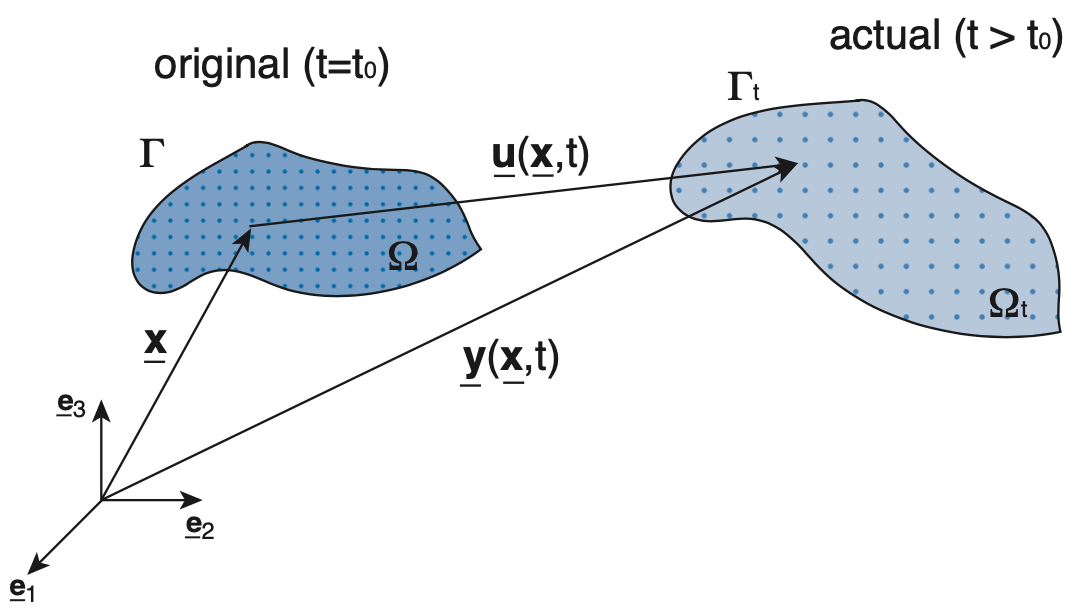
\includegraphics[width=0.5\linewidth]{img/Configurations} \\
\end{center}

\textbf{Final position:} {$\tensor[^i]{\underline{\mathbf{y}}}{} = {\underline{\underline{R}}} \tensor[^i]{\underline{\mathbf{x}}}{} + \underline{\mathbf{b}} \qquad i = 1,4 $} \\
With $ {\underline{\underline{R}}} = \left[\begin{array}{ccc}cos(\theta) & -sin(\theta) & 0 \\sin(\theta) & cos(\theta) & 0 \\0 & 0 & 1\end{array}\right]$ along axis $ \tensor[^3]{\underline{\mathbf{e}}}{}$ \ and $\quad \underline{\mathbf{b}} = \left[\begin{array}{c}0 \\0 \\n\end{array}\right]$ \\

Rotation matrix is \textbf{orthogonal}: $ {\underline{\underline{R^T}}} \underline{\underline{R}} = \underline{\underline{I}}$ \\

\textbf{Displacements:} {$ \tensor[^i]{\underline{\mathbf{u}}}{}(\underline{\mathbf{x}}, t) = \tensor[^i]{\underline{\mathbf{y}}}{}(\underline{\mathbf{x}}, t) - \tensor[^i]{\underline{\mathbf{x}}}{} \qquad i = 1,4 $} \\
\textbf{Velocities:} $\underline{\dot{\mathbf{y}}}(\underline{\mathbf{x}}, t) \equiv \diffp{\underline{\mathbf{y}}}{t}(\underline{\mathbf{x}}, t)$ \\
\textbf{Accelerations:} $\underline{\ddot{\mathbf{y}}}(\underline{\mathbf{x}}, t) \equiv \diffp[2]{\underline{\mathbf{y}}}{t}(\underline{\mathbf{x}}, t)$ \\


Motion is \textbf{bijective}: each beginning point has only $1$ ending point. This implies the existence of an inverse motion: $ \underline{y}^{-1} (\underline{y} (\underline{x},t),t) = \underline{x}$ \\

Rigid Body motion conserves volume: $ \Vert  \underline{y} - \underline{\tilde{y}} \Vert = \Vert  \underline{x} - \underline{\tilde{x}} \Vert$, but orientation is lost!

\lstinputlisting[style=Matlab-editor,basicstyle=\color{black}\ttfamily\normalsize, firstline=3, lastline=5]{CheatSheet.m}

\textbf{Gradient of displacement:} \\
$\underline{\underline{H}}(\underline{x},t) = \nabla_{\underline{x}} \underline{u} (\underline{x},t) = \left[\begin{smallmatrix} \frac{\delta u_1}{\delta x_1} & \frac{\delta u_1}{\delta x_2} & \frac{\delta u_1}{\delta x_3} \\ \frac{\delta u_2}{\delta x_1} & \frac{\delta u_2}{\delta x_2} & \frac{\delta u_2}{\delta x_3} \\ \frac{\delta u_3}{\delta x_1} & \frac{\delta u_3}{\delta x_2} & \frac{\delta u_3}{\delta x_3} \end{smallmatrix}\right] $\\
\textbf{Gradient of motion:}  $ \underline{\underline{F}} \rightarrow \underline{\underline{H}} = \underline{\underline{F}} - \underline{\underline{I}} $


$d \underline{u} = \underline{\underline{H}} d \underline{x} = \nabla_{\underline{x}} \underline{u} d \underline{x}$ \\
$= \underbrace{\frac{1}{2} (\underline{\underline{H}} + \underline{\underline{H}}^T)}_{\text{symmetric}} +  \underbrace{\frac{1}{2} (\underline{\underline{H}} - \underline{\underline{H}}^T)}_{\text{anti-symmetric}} $ \\
$= (\underline{\underline{\epsilon}} + \underline{\underline{A}}) d \underline{x} $


\subsection*{Coordinate System}
\smallskip

\textbf{Reference frame:} \begin{enumerate}
\item N points ($ N \geqslant 4 $ in 3D)
\item Non coplanar
\item Immobile
\item In fact, a \textbf{rigid body}
\end{enumerate}

\textbf{Orthogonal transformation $Q_{ij}$:} \\
A square matrix $\mathbf{Q}$ is \textit{orthogonal} if $\mathbf{Q}^{-1} = \mathbf{Q}^T$
\begin{itemize}
\item if $ \det{Q_{ij}} = +1$: orientation conserved;
\item if $ \det{Q_{ij}} = -1$: orientation inversed.
\end{itemize}

\textbf{Change into new CS:}
\begin{itemize}
\item Scalars $\alpha ' = \alpha$ $\rightarrow$ invariant
\item Vectors $v_i = Q_{ij}v_j$
\item Tensors of Order 2 $T'_{ij} = Q_{ik}Q_{jl}T_{kl}$
\end{itemize}

A \textbf{tensor of order n} is an object that needs n applications of the transformation $Q_{ij}$ to characterise the change of its components:
$C_{ij...n} '= Q_{ik} Q_{jl} ... Q_{nm} C_{kl...m}$ \\

\textbf{Isomorphism between $R^3$ × $R^3$ and $R^9$:} \\
$ \left[\begin{array}{ccc}T_{11} & T_{12} & T_{13} \\T_{21} & T_{22} & T_{23} \\T_{31} & T_{32} & T_{33}\end{array}\right] \leftrightarrow \left[\begin{array}{c}T_{11} \\T_{12} \\T_{13} \\T_{21} \\T_{22} \\T_{23} \\T_{31} \\T_{32} \\T_{33}\end{array}\right] $
\smallskip
\section{Homogeneous Transformations}
\subsection*{Dilatation}
\smallskip

\textbf{Homogeneous Dilatation:} {$\tensor[^i]{\underline{\mathbf{y}}}{} = \lambda (t/t_{max}) {\underline{\underline{\mathbf{I}}}} \tensor[^i]{\underline{\mathbf{x}}}{} \qquad i = 1,4 $} \\
with $ {\underline{\underline{\mathbf{I}}}} = \left[\begin{array}{ccc}1 & 0 & 0 \\0 & 1 & 0 \\0 & 0 & 1\end{array}\right]$
\lstinputlisting[style=Matlab-editor,basicstyle=\color{black}\ttfamily\normalsize, firstline=7, lastline=11]{CheatSheet.m}

\subsection*{Deformations}
\smallskip

\textbf{Uniaxial Deformation:}  {$\tensor[^i]{\underline{\mathbf{y}}}{}(t) = \underline{\underline{\mathbf{U}}} (t/t_{max})\tensor[^i]{\underline{\mathbf{x}}}{} \qquad i = 1,4 $} \\
$ \underline{\underline{U}}(t) = \underline{\underline{I}} + (\upsilon_a(t) -1) \underline{e}_1 \otimes \underline{e}_1 $ \\
with $ \underline{\underline{\mathbf{U}}} = \left[\begin{array}{ccc}1 & 0 & 0 \\0 & 1 & 0 \\0 & 0 & 2+t\end{array}\right]$ in case of a $300 \%$ deformation along $\tensor[^3]{e}{}$.
\smallskip

\textbf{Shear Deformation:}  {$\tensor[^i]{\underline{\mathbf{y}}}{}(t) = \underline{\underline{\mathbf{G}}} (t/t_{max})\tensor[^i]{\underline{\mathbf{x}}}{} \qquad i = 1,4 $} \\
Apply shear deformation ${\underline{\underline{\mathbf{G}}}}$ of ${\frac{\pi}{3}}$ along the vectors  $\tensor[^1]{e}{} - \tensor[^2]{e}{}$ linearly in time.
With det$\underline{\underline{\mathbf{G}}} = 1$ and $\underline{\underline{\mathbf{G}}} \neq \tensor[]{\underline{\underline{\mathbf{G}}}}{^T}$, which means that $\underline{\underline{\mathbf{G}}}$ contains a rotation.
\smallskip

\textbf{Simple shear:} $\underline{\underline{\mathbf{G}}}(t) = \underline{\underline{I}} + \tan{(\gamma (t))} (\underline{p} \otimes \underline{q})$ \\
$ \underline{\underline{\mathbf{G}}}(t) = \left[\begin{array}{ccc}1 & \tan (\gamma) & 0 \\0 & 1 & 0 \\0 & 0 & 1\end{array}\right]$ \\
$ \det{\underline{\underline{\mathbf{G}}}} = 1 \rightarrow $ no change of volume, rotation!

\textbf{Pure shear:} $\underline{\underline{U}} = \underline{\underline{U}}^T \rightarrow $ no rotation! \\
$ \underline{\underline{\mathbf{G}}}(t) = \left[\begin{array}{ccc}1 & \frac{1}{2} \tan (\gamma) & 0 \\ \frac{1}{2} \tan (\gamma) & 1 & 0 \\0 & 0 & 1\end{array}\right]$ \\

\textbf{General Deformation:} \\
Volume change: $V_t = \operatorname{det}(\underline{\underline{\mathbf{F}}}) V $ \\
Area-weighted normals of the tetrahedron: 
$\tensor[^i]{A}{_t} \tensor[^i]{\underline{\mathbf{n}}}{_t} = \operatorname{det}(\underline{\underline{\mathbf{F}}}) \tensor[]{\underline{\underline{\mathbf{F}}}}{^{-T}} \tensor[^i]{A}{} \tensor[^i]{\underline{\mathbf{n}}}{}$
\smallskip
Apply general deformation: {$\tensor[^i]{\underline{\mathbf{y}}}{}(t) = \underline{\underline{\mathbf{F}}} (t/t_{max})\tensor[^i]{\underline{\mathbf{x}}}{} \qquad i = 1,4 $}\\
Where $\underline{F}$ is the Fréchet derivative of a motion (represents rotation, deformation, translation). \\

\textbf{Gradient of transformation:} The infinitesimal transformations of a fiber $da$, surface $ds$ and volume $dV$ are given by: \\

$ d \underline{a}_t = \underline{\underline{F}} d \underline{a} $ \\
$ d \underline{s}_t = J \underline{\underline{F}} ^{-T} d \underline{s} = \underline{\underline{F}}^* d \underline{s}$ \\
$ d V_t = \det{\underline{\underline{F}}} dV = JdV $ \\
With $F^* = j \cdot \underline{\underline{F}} ^{-T} =  \det({\underline{\underline{F}}}) \cdot \underline{\underline{F}} ^{-T}$ \\

$\underline{\underline{\mathbf{F}}}(\underline{\mathbf{x}},t) = \underline{\underline{\mathbf{H}}}(\underline{\mathbf{x}},t) + \underline{\underline{\mathbf{I}}} = \left[\begin{smallmatrix} \frac{\delta y_1}{\delta x_1} & \frac{\delta y_1}{\delta x_2} & \frac{\delta y_1}{\delta x_3} \\ \frac{\delta y_2}{\delta x_1} & \frac{\delta y_2}{\delta x_2} & \frac{\delta y_2}{\delta x_3} \\ \frac{\delta y_3}{\delta x_1} & \frac{\delta y_3}{\delta x_2} & \frac{\delta y_3}{\delta x_3} \end{smallmatrix}\right]$ \\

\medskip
Properties of $ \mathbf{\underline{\underline{F}}}: $
\begin{enumerate}
\item $ \underline{\underline{F}} \neq \underline{\underline{F}}^T $: usually \underline{\underline{F}} is not symmetric.
\item $0 < \det{\underline{\underline{F}}} < \infty $
\item $\underline{\underline{F}}^{-1} \underline{\underline{F}} = \underline{\underline{I}}$
\item if $J(\underline{\mathbf{x}},t) = 1$, $\rightarrow$ \textbf{incompressible} (isochoric)
\end{enumerate}
The Jacobian $J(x,t)$ of the transformation is the change of volume of an infinitesimal element at point \underline{x}. \\

\textbf{Cayley-Hamilton} claims that each tensor of Order 2 satisfies: \\
$\underline{\underline{\mathbf{F}}}^3 - \Tr({\underline{\underline{\mathbf{F}}}}) \underline{\underline{\mathbf{F}}}^2 + \Sec({\underline{\underline{\mathbf{F}}}}) \underline{\underline{\mathbf{F}}} - \det({\underline{\underline{\mathbf{F}}}}) \underline{\underline{\mathbf{I}}} = \underline{\underline{\mathbf{0}}}$ \\
The 3 consecutive powers of $\underline{\underline{\mathbf{F}}}$ having the same eigenvectors are related by their singular values. \\

\textbf{Polar Decomposition:} $ \underline{\underline{F}} = \underline{\underline{R}} \underline{\underline{U}} = \underline{\underline{V}} \underline{\underline{R}} $, where: \\
$\underline{\underline{U}}$ : \textbf{right} stretch tensor (pos, def, symm.) $ \hspace{8mm} \sqrt{\underline{\underline{F}}^T \underline{\underline{F}}} $ \\ 
$\underline{\underline{V}}$ : \textbf{left} stretch tensor (pos, def, symm.) $ \hspace{10mm} \sqrt{\underline{\underline{F}} \underline{\underline{F}}^T} $ \\

\begin{center}
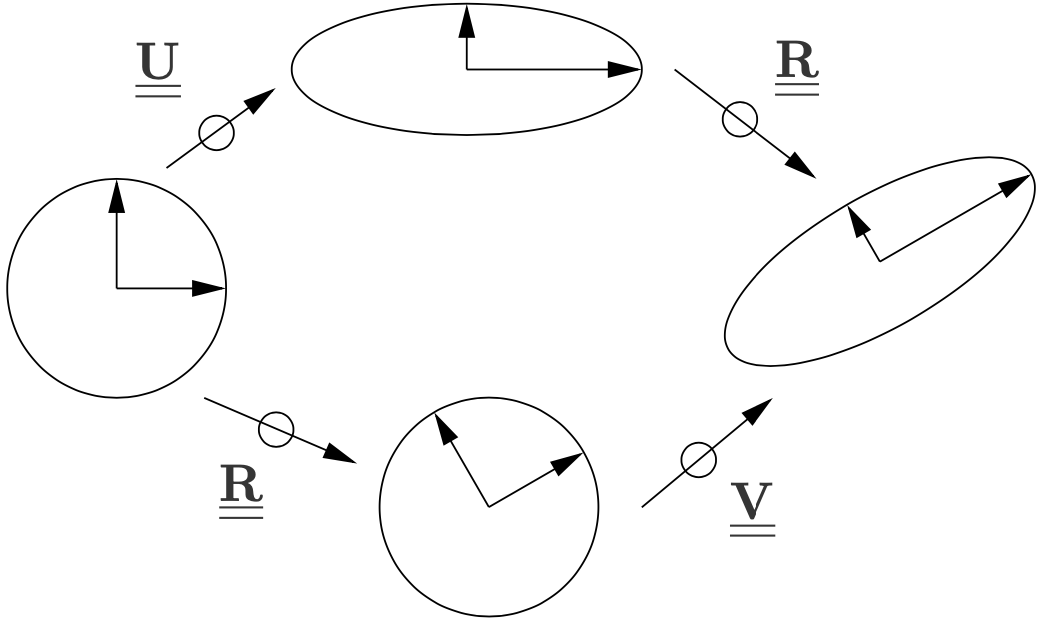
\includegraphics[width=0.6\linewidth]{img/PolarDecomp} \\
\end{center}

\textbf{Singular decomposition:} $ \underline{\underline{F}} =  \sum_{a=1}^{3} \upsilon_a (\underline{b}_a \otimes \underline{c}_a) $, with: \\
$\upsilon_a$: singular values of $\underline{\underline{F}}$ \quad $ 0 < \upsilon_a < \infty$ \quad $\underline{b}_a = \underline{\underline{R}} \underline{c}_a $ \quad $ \underline{c}_a \cdot \underline{c}_b = \delta_{ab} $ \\

The \textbf{invariants} of the gradient of the transformation can be expressed in terms of the singular values: \\
$\Tr{\underline{\underline{F}}(\underline{x},t)} = \sum_{a=1}^{3} \upsilon_a$ \\
$\Sec{\underline{\underline{F}}(\underline{x},t)} = \sum_{a=1}^{3} \upsilon_a \upsilon_b $ \\
$\det{\underline{\underline{F}}(\underline{x},t)} = \prod_{a=1}^{3} \upsilon_a $ \\


\textbf{Spectral decomposition:} states that a symmetric, strictly positive definite tensor ${\underline{\underline{\mathbf{U}}}}$ can be expressed as:

${\underline{\underline{\mathbf{U}}}} = \sum \limits_{a=1}^{3} v_a (\mathbf{\underline{c}}_{a} \otimes \mathbf{\underline{c}}_{a})$ \\

\textbf{Unimodular decomposition:} states that ${\underline{\underline{\mathbf{F}}}}$ can be decomposed in a spherical compression or dilatation ${\underline{\underline{\mathbf{J}}}}$ and an isovolumic deformation ${\underline{\underline{\mathbf{\hat{F}}}}}$ \\

${\underline{\underline{\mathbf{F}}}} = {\underline{\underline{\mathbf{J}}}} {\underline{\underline{\mathbf{\hat{F}}}}} = {\underline{\underline{\mathbf{\hat{F}}}}} {\underline{\underline{\mathbf{J}}}}$ \\
${\underline{\underline{\mathbf{J}}}} = J^{\frac{1}{3}}  {\underline{\underline{\mathbf{I}}}}$ \\


\textbf{Infinitesimal Strain tensor:} \\
${\underline{\underline{\mathbf{\epsilon}}}} = \frac{1}{2}({\underline{\underline{\mathbf{H}}}}+{\underline{\underline{\mathbf{H}}}}^T)$ \\
Relative volume change is approximated by: \\
$\frac{\Delta V}{V} \cong \Tr({{\underline{\underline{\mathbf{\epsilon}}}}})$

\smallskip
\section{Alternative Strains}
\subsection*{Cauchy-Green tensors}
\smallskip

\textbf{Right Cauchy-Green strain tensor:} $\rightarrow$ Material tensor \\
$\underline{\underline{C}} = \tensor[]{\underline{\underline{F}}}{^T} \underline{\underline{F}} = \underline{\underline{U}}^2 $ \\
Where $\underline{\underline{C}} = \tensor[]{\underline{\underline{C}}}{^T} \rightarrow $ symmetric, positive definite and filters the rotation appearing in polar decomp. of $\underline{\underline{\mathbf{F}}}$ \\
$ \underline{\underline{\mathbf{C}}} = \sum \limits_{a=1}^{3} \upsilon_{a}^{2} (\underline{c}_a \otimes \underline{c}_a) $



\textbf{Left Cauchy-Green strain tensor:} $\rightarrow$ Spatial tensor \\
$\rightarrow$ Maps the actual configuration into itself. \\
$\underline{\underline{B}} = \underline{\underline{F}} \tensor[]{\underline{\underline{F}}}{^T} = \underline{\underline{V}}^2$ \\
Where $\underline{\underline{B}} = \tensor[]{\underline{\underline{B}}}{^T}$ \\
\smallskip

\subsection*{Green-Lagrange strain tensor}
\smallskip
Objective transformation that shifts the absence of deformation from $\underline{\underline{\mathbf{I}}}$ to $\underline{\underline{\mathbf{0}}}$. \\
$ \mathbf{\underline{\underline{E}}} = \mathbf{\frac{1}{2}(\underline{\underline{C}} - \underline{\underline{I}})}  = \underbrace{\frac{1}{2} (\underline{\underline{H}} + \underline{\underline{H}}^T)}_{\text{$\epsilon$}} +  \underline{\underline{HH}}^T$, \qquad
where $\underline{\underline{E}} = \tensor[]{\underline{\underline{E}}}{^T}$. \\
When $\mathbf{\underline{\underline{E}}} =0$: rigid body motion (reduction to zero tensor when there is no deformation).

\subsection*{Hill strain tensor}
\smallskip

$ \underline{\underline{E}}_h = \sum \limits_{a=1}^{3} h(\upsilon_{a}) (\underline{c}_a \otimes \underline{c}_a) $ \\
Where $h(\upsilon)$ is a strictly increasing scalar function. \\


\subsection*{Logarithmic strain tensor}
\smallskip

$ \ln{\underline{\underline{U}}} = \sum \limits_{a=1}^{3} \ln{(\upsilon_{a})} (\underline{c}_a \otimes \underline{c}_a) $ \qquad from \textbf{right} stretch tensor\\
$ \ln{\underline{\underline{V}}} = \sum \limits_{a=1}^{3} \ln{(\upsilon_{a})} (\underline{b}_a \otimes \underline{b}_a) $ \qquad from \textbf{left} stretch tensor \\


\subsection*{Strain rates}
\smallskip
\textbf{Rate of the gradient of the transformation:} gradient of the velocity field. \\ \smallskip
$\underline{\underline{\dot{\mathbf{F}}}} = \dod{\underline{\underline{\mathbf{F}}}}{t}$ \\

Right Cauchy-Green strain rate tensor: \\
$\underline{\underline{\dot{\mathbf{C}}}} = \underline{\underline{\dot{\mathbf{F}}}}^T \underline{\underline{\mathbf{F}}} + \underline{\underline{\mathbf{F}}}^T \underline{\underline{\dot{\mathbf{F}}}}$ \\

Green-Lagrange strain rate tensor: \\
$ \underline{\underline{\dot{\mathbf{E}}}} = \frac{1}{2} \underline{\underline{\dot{\mathbf{C}}}}$

\textbf{Spatial strain rate:} \\ Left Cauchy-Green strain rate \\
$ \underline{\underline{\dot{\mathbf{B}}}} = \underline{\underline{\dot{\mathbf{F}}\mathbf{F}}}^T + \underline{\underline{\mathbf{F}\mathbf{\dot{F}}}}^T$


\smallskip
\textbf{Eulerian deformation rate:} $\frac{1}{2}(\nabla_y v + \nabla_y^T v)$ \\

$ \underline{\underline{\mathbf{D}}}(\underline{\mathbf{y}},t) = \frac{1}{2}( \underline{\underline{\mathbf{L}}}(\underline{\mathbf{y}},t) +  \underline{\underline{\mathbf{L}}}^T(\underline{\mathbf{y}},t))$ \\
With the spatial gradient of the velocity field $\underline{\underline{\mathbf{L}}}(\underline{\mathbf{y}},t)$ :\\
$\underline{\underline{\mathbf{L}}}(\underline{\mathbf{y}},t) = \underline{\underline{\mathbf{\dot{F}}}}(\underline{\mathbf{x}},t) \underline{\underline{\mathbf{F}}}^{-1}(\underline{\mathbf{y}},t) $

\textbf{Formula connecting Eulerian and Lagrangean deformation rates:} \\
$ \underline{\underline{D}} = \underline{\underline{F}}^{-T} \underline{\underline{\dot{E}}}  \underline{\underline{F}}^{-1}  $ \\




\subsection*{Change of Coordinate System}
\smallskip

A change of coordinate system involves a time-independent transformation $\underline{\underline{\mathbf{Q}}}$ of the base vectors and a time-independent translation $\underline{\mathbf{q}}$ of the origin. \\

$\underline{\mathbf{\underline{Q}}} = \tensor[^3]{\underline{\mathbf{\underline{R}}}}{}(\frac{\pi}{12}) \tensor[^2]{\underline{\mathbf{\underline{R}}}}{}(\frac{\pi}{9}) \tensor[^1]{\underline{\underline{\mathbf{R}}}}{}(\frac{\pi}{6})$
$ \qquad \underline{\mathbf{q}} = - \frac{1}{8} \tensor[^3]{\underline{\mathbf{e}}}{}$

Where $\underline{\mathbf{\underline{Q}}}$ and ${\mathbf{\underline{q}}}$ are the orthogonal transformation: \\
$\underline{\mathbf{\underline{Q}}}$: Translation applying the current base vectors, \\
${\mathbf{\underline{q}}}$: Current origin into the new base vectors. \\

A vector $\underline{\mathbf{x}}$ in the new system is: $\underline{\mathbf{\tilde{x}}} = \tensor[]{\underline{\underline{\mathbf{Q}}}}{^T}(\underline{\mathbf{x}} - \underline{\mathbf{q}})$
($\underline{\mathbf{\underline{Q}}}$ and ${\mathbf{\underline{q}}}$ expressed in initial C.S.).

\subsection*{Objectivity}
($=$ frame indifference) \\
Property of invariance of a law with respect to a general change of reference frame. Any physical quantity with an intrinsic feature must be invariant relative to a particular change of observer.\\


%\begin{table}{ccc}
%  \centering 
%\textbf{Spatial} & \textbf{Material} & \textbf{Nominal} \\
%\hline
% $\hat{\phi} = \phi(\underline{y}) $ & $ \hat{\phi}(\underline{\hat{y}}) = \phi(\underline{x}) $ & $\phi(\underline{x})$ \\
% \hline
%\end{table}

\begin{tabular} {>{\centering\arraybackslash}m{2.7cm}>{\centering\arraybackslash}m{2.8cm}>{\centering\arraybackslash}m{2.7cm}}
\toprule
\textbf{Spatial} & \textbf{Material} & \textbf{Nominal} \\
\midrule
 $\hat{\phi} = \phi(\underline{y}) $ & $ \hat{\phi}(\underline{\hat{y}}) = \phi(\underline{x}) $ & $\phi(\underline{x})$ \\
\midrule

 $\underline{\hat{\upsilon}_t} (\underline{\hat{x}}, \hat{t}) = \underline{\underline{Q}}^T \underline{\upsilon}_t (\underline{y},t)$ & $\underline{\hat{\upsilon}_t} (\underline{\hat{x}}, \hat{t}) = \underline{\upsilon}_t (\underline{x},t)$ & $\underline{\underline{Q}}^T \underline{\upsilon}_t (\underline{x},t) $\\
\midrule
 
$\underline{\underline{\mathbf{B}}}$ & $\underline{\underline{\mathbf{E}}}; \underline{\underline{\mathbf{C}}} $& $ \underline{\underline{\mathbf{F}}}$ \\
\bottomrule
\end{tabular}
\smallskip

Detailed explanation: \\
$\underline{\underline{\hat{B}}} (\underline{\hat{y}}, \hat{t}) = \underline{\underline{Q}}^T $ $ \underline{\underline{B}} $  $\underline{\underline{Q}}$ \\
$ \underline{\underline{\hat{\mathbf{F}}}} = \underline{\underline{Q}}^T \underline{\underline{F}}$

\subsection*{Velocity}
\smallskip

The velocity resulting from a general change of ref. frame is: \\

$ \dot{\hat{\underline{y}}} = \underbrace{\underline{\underline{Q}}^T \dot{\underline{y}}}_{\text{relative velocity}} + \underbrace{\underline{\underline{\dot{Q}}}^T \underline{y} + \dot{\underline{q}}}_{\text{rate of relative rotation}} $ \\
Observers are located at different places in space and move relative to each other, as implied by the time-dependence of $\mathbf{c}(t)$ and $\mathbf{Q}(t)$. Therefore, the descriptions of motions depend on the observers and, consequently, the velocity and acceleration of motion are, in general, \textbf{not objective}.
Velocity is objective only when the change of reference frame is time independent! \\

\subsection*{Acceleration}
\smallskip

The acceleration resulting from a general change of ref. frame is: \\

$ \ddot{\hat{\underline{y}}} = \underbrace{\underline{\underline{Q}}^T \ddot{\underline{y}}}_{\text{Relative acceleration}} + \underbrace{2\underline{\underline{\dot{Q}}}^T \underline{\dot{y}}}_{\text{Coriolis acceleration}} + \underbrace{\underline{\underline{\ddot{Q}}}^T \underline{y} + {\underline{\ddot{q}}}}_{\text{Centrifugal acceleration}} $ \\


\subsection*{Lagrangean descriptions}
\smallskip
Within the Lagrangean description, distinction between nominal (mixed), spatial (updated) and material (total) Lagrangean description is made. \\

\textbf{Nominal description}: the control volume and its related dimensions are referred to the \textbf{original configuration} $\Omega$. Forces $\underline{f}_t$ (applied by nature in the actual configuration
$\Omega_t$) are expressed in original positions via the motion $ \underline{f}_t \circ \underline{y}$. \\

\textbf{Spatial Lagrangean description:} the control volume and all related dimensions are referred to the \textbf{actual configuration} $\Omega_t$, and the applied forces are again expressed in the previous positions via the motion. \\

\textbf{Material Lagrangean description:} the control volume and all related dimensions are also referred to the \textbf{original configuration} $\Omega$, but the applied forces are transformed by some function of the motion in order to be defined on the original configuration $\Omega$ and respect a principle of duality. \\
\smallskip
\section{Mass and Density}
\subsection*{Face geometrical centers}
\smallskip

$\tensor[^{cf1}]{\underline{\mathbf{x}}}{} = 2 \mathlarger{\int_{0}^{1} \int_{0}^{1-\tensor[^3]{b}{}} (\tensor[^2]{b}{} \tensor[^2]{\underline{\mathbf{x}}}{}) + \tensor[^3]{b}{} \tensor[^3]{\underline{\mathbf{x}}}{} + (1 - \tensor[^2]{b}{} - \tensor[^3]{b}{}) \tensor[^4]{\underline{\mathbf{x}}}{}) d \tensor[^2]{b}{}d \tensor[^3]{b}{}}$ \\


$\tensor[^{cf2}]{\underline{\mathbf{x}}}{} = 2 \mathlarger{\int_{0}^{1} \int_{0}^{1-\tensor[^3]{b}{}} (\tensor[^1]{b}{} \tensor[^1]{\underline{\mathbf{x}}}{}) + \tensor[^3]{b}{} \tensor[^3]{\underline{\mathbf{x}}}{} + (1 - \tensor[^1]{b}{} - \tensor[^3]{b}{}) \tensor[^4]{\underline{\mathbf{x}}}{}) d \tensor[^1]{b}{}d \tensor[^3]{b}{}}$ \\

$\tensor[^{cf3}]{\underline{\mathbf{x}}}{} = 2 \mathlarger{\int_{0}^{1} \int_{0}^{1-\tensor[^2]{b}{}} (\tensor[^1]{b}{} \tensor[^1]{\underline{\mathbf{x}}}{}) + \tensor[^2]{b}{} \tensor[^2]{\underline{\mathbf{x}}}{} + (1 - \tensor[^1]{b}{} - \tensor[^2]{b}{}) \tensor[^4]{\underline{\mathbf{x}}}{}) d \tensor[^1]{b}{}d \tensor[^2]{b}{}}$ \\

$\tensor[^{cf4}]{\underline{\mathbf{x}}}{} = 2 \mathlarger{\int_{0}^{1} \int_{0}^{1-\tensor[^2]{b}{}} (\tensor[^1]{b}{} \tensor[^1]{\underline{\mathbf{x}}}{}) + \tensor[^2]{b}{} \tensor[^2]{\underline{\mathbf{x}}}{} + (1 - \tensor[^1]{b}{} - \tensor[^2]{b}{}) \tensor[^3]{\underline{\mathbf{x}}}{}) d \tensor[^1]{b}{}d \tensor[^2]{b}{}}$ \\

\subsection*{Face normals}
\smallskip

$\tensor[^1]{\underline{\mathbf{n}}}{} = \frac{(\tensor[^3]{\underline{\mathbf{x}}}{} - \tensor[^4]{\underline{\mathbf{x}}}{}) \wedge
(\tensor[^2]{\underline{\mathbf{x}}}{} -\tensor[^4]{\underline{\mathbf{x}}}{})}{\|(\tensor[^3]{\underline{\mathbf{x}}}{} - \tensor[^4]{\underline{\mathbf{x}}}{}) \wedge
(\tensor[^2]{\underline{\mathbf{x}}}{} -\tensor[^4]{\underline{\mathbf{x}}}{})\|}$ \\

$\tensor[^2]{\underline{\mathbf{n}}}{} = \frac{(\tensor[^3]{\underline{\mathbf{x}}}{} - \tensor[^4]{\underline{\mathbf{x}}}{}) \wedge
(\tensor[^1]{\underline{\mathbf{x}}}{} -\tensor[^4]{\underline{\mathbf{x}}}{})}{\|(\tensor[^3]{\underline{\mathbf{x}}}{} - \tensor[^4]{\underline{\mathbf{x}}}{}) \wedge
(\tensor[^1]{\underline{\mathbf{x}}}{} -\tensor[^4]{\underline{\mathbf{x}}}{})\|}$ \\

$\tensor[^3]{\underline{\mathbf{n}}}{} = \frac{(\tensor[^2]{\underline{\mathbf{x}}}{} - \tensor[^4]{\underline{\mathbf{x}}}{}) \wedge
(\tensor[^1]{\underline{\mathbf{x}}}{} -\tensor[^4]{\underline{\mathbf{x}}}{})}{\|(\tensor[^2]{\underline{\mathbf{x}}}{} - \tensor[^4]{\underline{\mathbf{x}}}{}) \wedge
(\tensor[^1]{\underline{\mathbf{x}}}{} -\tensor[^4]{\underline{\mathbf{x}}}{})\|}$ \\

$\tensor[^4]{\underline{\mathbf{n}}}{} = \frac{(\tensor[^3]{\underline{\mathbf{x}}}{} - \tensor[^2]{\underline{\mathbf{x}}}{}) \wedge
(\tensor[^1]{\underline{\mathbf{x}}}{} -\tensor[^3]{\underline{\mathbf{x}}}{})}{\|(\tensor[^3]{\underline{\mathbf{x}}}{} - \tensor[^2]{\underline{\mathbf{x}}}{}) \wedge
(\tensor[^1]{\underline{\mathbf{x}}}{} -\tensor[^3]{\underline{\mathbf{x}}}{})\|}$ \\

\subsection*{Volume, Mass, C.o.G}
\smallskip

\textbf{Volume of the tetrahedron:} $ V = \frac{1}{6} (\tensor[^3]{\underline{\mathbf{x}}}{} - \tensor[^4]{\underline{\mathbf{x}}}{}) \cdot \left[ (\tensor[^1]{\underline{\mathbf{x}}}{} -\tensor[^4]{\underline{\mathbf{x}}}{}) \wedge (\tensor[^2]{\underline{\mathbf{x}}}{} -\tensor[^4]{\underline{\mathbf{x}}}{})  \right]$

\textbf{Mass of the tetrahedron:} $M = 6 \rho V$ \\


\textbf{Center of Gravity:}

 $\tensor[^c]{\underline{\mathbf{x}}}{} = \frac{6V}{M}  \mathlarger{\int_{0}^{1} \int_{0}^{1-\tensor[^3]{b}{}} \int_{0}^{1-\tensor[^2]{b}{} - \tensor[^3]{b}{}}} \underline{\mathbf{x}} (\tensor[^1]{b}{}, \tensor[^2]{b}{}, \tensor[^3]{b}{}) \rho d \tensor[^1]{b}{} d \tensor[^2]{b}{} d \tensor[^3]{b}{} $ \\
 
 \subsection*{Tensor of mass and Tensor of inertia:}
\smallskip
\textbf{Mass} is a scalar, positive, additive. \\
$M_t(\Omega_t, t) = \int_{\Omega_t} \rho_t dV_t > 0$ \\
\smallskip
\textbf{Conservation of mass:} $\rho_t(\underline{\mathbf{y}}, t) = \rho J^{-1}(\underline{\mathbf{y}},t)$ \\
Tensor of mass $\tensor[^c]{\underline{\underline{M}}}{}(\Omega, t)$ with respect to the CoM.\\

Tensor of inertia $\tensor[^c]{\underline{\underline{J}}}{}(\Omega, t)$ [\si{\kg\metre\squared}]with respect to the CoM. \\

\textbf{Huygens-Steiner:} $\tensor[^o]{\underline{\underline{J}}}{} = M ((\underline{c} \cdot \underline{c}) \underline{\underline{I}} - \underline{c} \otimes \underline{c}) + \tensor[^c]{\underline{\underline{J}}}{} $ \\

\textbf{Moment of inertia} in a plane normal to direction $\underline{\mathbf{n}}$ wrt CoM: \\
$\tensor[^c]{\underline{\underline{m}}}{}(\Omega, t, \underline{\mathbf{n}}) = \underline{\mathbf{n}} \cdot  \tensor[^c]{\underline{\underline{J}}}{}(\Omega, t)\underline{\mathbf{n}}$

\textbf{Radius of gyration:} $ \tensor[^c]{r}{^G}(\Omega, t, \underline{n}) = \sqrt{\frac{\tensor[^c]{m}{}(\Omega, t, \underline{n})} {M(\Omega, t)} }$ \\
"Radius at which a concentrated mass leads to an equivalent moment of inertia" \\
\smallskip
\section{Inertial and Volume Forces}
\subsection*{Linear and angular momentum}
\smallskip

\textbf{Linear momentum} (formulate the forces and moments associated with inertial effects) \\
$ \underline{l}(\Omega, t) = M(\Omega) \dot{\underline{c}}(\Omega, t) $ \qquad where $\dot{\underline{c}}$ is the spatial velocity field of the \textbf{centre of mass}. \\

\textbf{Angular momentum:} \\
\textit{Reference to Origin:} \\
$ \tensor[^o]{\hat{\underline{J}}}{} = \int_{\Omega} \underline{y} \wedge \dot{\underline{y}} \rho dV $ \\

\textit{Reference to CoM:} \\
$ \tensor[^c]{\hat{\underline{l}}}{} (\Omega, t) = \int_{\Omega} \underbrace{(\underline{y} - \underline{c})}_{\text{lever arm}} \wedge \dot{\underline{y}} \rho dV $ \\

\textbf{Theorem of König:} \\
$ \tensor[^o]{\hat{\underline{l}}}{} (\Omega, t) = \underbrace{\tensor[^c]{\hat{\underline{l}}}{}}_{\text{Intrinsic}} + \underbrace{\underline{c} \wedge \underline{l}}_{\text{Extrinsic, wrt O}} $ \\

\textbf{Instantaneous velocity of rotation:} \\
$\underline{\mathbf{\omega}}(t) = -\frac{1}{2} \underline{\underline{\underline{\mathbf{\epsilon}}}} \underline{\underline{\mathbf{\dot{R}}}} \underline{\underline{\mathbf{R}}}^T$

\textbf{Inertial mass} of 0th order, expressing proportionality between the linear momentum and the translation velocity. \\
\textbf{Tensor of inertia} of 2nd order and characterises the proportionality between the intrinsic angular momentum and the rotational velocity about the same point. \\

\subsection*{Inertial forces and moments}
\smallskip
The forces and the moments with respect to the origin that are opposed to the change of velocity of a deformable body are defined by the material derivatives of the linear and angular momentum respectively: \\

$ \diff{\underline{\mathbf{l}}}{t}(\Omega, t) = \int_{\Omega} \ddot{\underline{\mathbf{y}}} \rho dV$ \\
$\diff{^{o}\underline{\mathbf{\hat{I}}}}{t} (\Omega, t) = \int_{\Omega} \underline{\mathbf{y}} \wedge \ddot{\underline{\mathbf{y}}} \rho dV$ \\

\subsection*{Volume forces}
\smallskip
Such as gravitational or magnetic forces, act remotely and through the considered tissue. \\
$ \underline{\mathbf{k}}(\Omega, t): \int_{\Omega} \underline{\mathbf{\kappa}}(\underline{x},t) dV $ (Force per unit Vol.) \\
$ ^{o}\underline{\mathbf{\hat{k}}} = \int_{\Omega} \underline{y} (\underline{x},t) \wedge \underline{\mathbf{\kappa}}(\underline{x},t) dV $ \\

\textbf{Gravitational field:} $\underline{\mathbf{\kappa}}(\underline{x},t) = - \rho (\underline{x},t) g \underline{\tensor[]{e}{_3}} $ With $g = 9.81 [\frac{m}{s^2}]$ \\
The \textbf{density} of a volume force is derived from the spatial density:
$\underline{\mathbf{\kappa}}(\underline{x},t) = \tensor[]{\underline{\mathbf{\kappa}}}{_t}(\underline{y},t) \cdot J(\underline{x},t) $ \\
\textbf{Contact moment:} $\tensor[^o]{\hat{\underline{q}}}{_t} (\omega_o, t) = \int_{\Gamma} \underline{y} \wedge \underline{p} (\underline{x},t) dA $ \\

\columnbreak
 
\subsection*{Contact forces and moments}
\smallskip
Distributed on the surface. In nominal description, the force and the moment of the actual contact $\underline{\mathbf{q}}$ and $\underline{\mathbf{\hat{q}}}$ are defined by integration of the nominal stress vector $\underline{\mathbf{p}}$ (PK1) over the original surface. \\
$\underline{q} (\Gamma,t) = \int_{\Gamma} \underline{p}(\underline{x},t)dA$ \\

Contact force = Inertial force - Volume force: \\
$\underline{p} = \rho \underline{\ddot{y}} - \underline{k}$ \\

Nominal stress vector due to hydrostatic pressure generally NOT normal to the original surface: \\
$\Pi (\underline{x},t) = \Pi (\underline{y},t) \circ \underline{y} (\underline{x},t)$ \\

Balance of linear momentum: \\
$\underbrace{\int \rho \underline{\mathbf{b}} d V}_{\text{vol-f}} + \underbrace{\int \underline{\mathbf{t}} ds}_{\text{con-f}}  = \underbrace{\frac{d}{dt} \int \rho \underline{\mathbf{v}} dV}_{\text{ine-f}} $ \\

\textbf{Force vectors $\tensor[^i]{f}{}$:} \\
$\tensor[^i]{\underline{\mathbf{f}}}{}(t) = - \frac{1}{3} \left[ \underline{\mathbf{I}}(t) + \underline{\mathbf{W}}(t) \right] \tensor[^i]{A}{_t}(t) \tensor[^i]{\underline{\mathbf{n}}}{}(t) + \frac{1}{4} \tensor[^{con}]{\underline{\mathbf{f}}}{}(t)$ \\
\section{Stresses}
\subsection*{Internal Forces}
\smallskip

Internal cohesive forces are at the origin of the stresses responsible for deformations. Modeling of these forces requires 2 hypotheses: \\

\begin{enumerate}
\item Cohesive force distributed over the surface $\partial \omega$ of the sub-domain
\item Nominal stress vector only depends on the orientation of the surface in $\underline{\mathbf{x}} \rightarrow$ because PK1 is measured in original configuration! 
\end{enumerate}


\subsection*{Stresses}
\smallskip

\fbox{%
    \parbox{\columnwidth}{%
\textbf{Nominal stress tensor:} \hspace{8mm} Piola-Kirchhof 1 ($\underline{\underline{\mathbf{P}}}$)\\
\textbf{Spatial stress tensor:} \hspace{10mm} Cauchy (true) ($\underline{\underline{\mathbf{T}}}$)\\
\textbf{Material stress tensor:} \hspace{8mm} Piola-Kirchhof 2 ($\underline{\underline{\mathbf{S}}}$)
    }%
}

\begin{center}
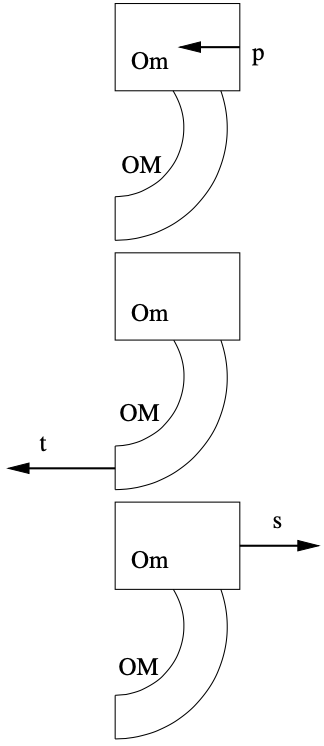
\includegraphics[width=0.3\linewidth]{img/StressVectors} \\
\end{center}

\textbf{Nominal stress tensor:} $ \underline{p} = \underline{\underline{P}} (\underline{x},t) \underline{n}(\underline{x})$ Where $\underline{\underline{P}} \neq$ symm! \\

\textbf{Spatial stress tensor:} (=Cauchy stress tensor)\\
$ \underline{\underline{T}} = J^{-1} \underline{\underline{P}} \underline{\underline{F}}^T$ \\
$ \underline{\underline{P}} = \underline{\underline{T}} \underline{\underline{F}}^*$ \\
$ = \underline{\underline{T}} \det(\underline{\underline{F}}) \cdot \underline{\underline{F}}^{-T}$

Nominal and Cauchy stress tensors are sensitive to rotations. \\
\textbf{Rates are NOT objective} \\


\textbf{Material stress tensor:} symmetric, objective, filters rigid body motions \\
$ \underline{\underline{\mathbf{P}}}(\underline{x}, t) = \underline{\underline{\mathbf{F}}}(\underline{x}, t) \underline{\underline{\mathbf{S}}}(\underline{x}, t)$ \\
3 invariants: \\
$I_1 = \Tr{\underline{\underline{S}}} = \sigma_1 + \sigma_2 + \sigma_3$ \\
$I_2 = \Sec{\underline{\underline{S}}} = \sigma_{2}\sigma_3 + \sigma_3\sigma_1 + \sigma_1\sigma_2 $ \\
$I_3 = \det{\underline{\underline{S}}} = \sigma_1\sigma_2\sigma_3$\\

\textbf{Stress tensors:} \\
$\underline{\underline{T}} = J^{-1} \underline{\underline{F}} \underline{\underline{S}} \underline{\underline{F}}^T$ \\
$\underline{\underline{S}} = J \underline{\underline{F}}^{-1} \underline{\underline{T}} \underline{\underline{F}}^{-T}$

Decompose \textbf{Stress tensor} in \textbf{Hydrostatic} and \textbf{Deviatoric} parts: \\
$\underline{\underline{\mathbf{S}}} = \underbrace{\frac{1}{3} \Tr{\underline{\underline{S}}}}_{\text{Hydr. P}} \underline{\underline{I}} + \underbrace{\underline{\underline{S}}'}_{\text{deviatoric part}}$ \\

\textbf{Stress deviator}: \\
$\underline{\underline{\mathbf{S}}}' = \underline{\underline{\mathbf{S}}} - \frac{1}{3}\Tr({\underline{\underline{\mathbf{S}}}}) \underline{\underline{\mathbf{I}}}$ \\

\textbf{Invariants of stress deviator}: \\
\begin{enumerate}
\item $J_1 = \Tr({\underline{\underline{\mathbf{S}}}}') = 0$
\item $J_2 = \frac{1}{2} \Tr({\underline{\underline{\mathbf{S}}}}'^2) = 0$
\item $J_3 = \frac{1}{3} \Tr({\underline{\underline{\mathbf{S}}}}'^3) = 0$
\end{enumerate}

\textbf{Von Mises stress:} Norm of the deviatoric part of the stress \\
$\tensor[^{vM}]{S}{} = \sqrt{\frac{3}{2} \underline{\underline{\mathbf{S'}}} : \underline{\underline{\mathbf{S'}}}} = \sqrt{3 J_2} = \sqrt{\frac{3}{2} \Tr({\underline{\underline{\mathbf{S}}}}'^2)}$ \\
With $\underline{\underline{\mathbf{S'}}} = \underline{\underline{\mathbf{S}}} + \pi \underline{\underline{\mathbf{I}}}$

\textbf{Hydrostatic Pressure:} $\pi = - \frac{1}{3} \operatorname{tr}\underline{\underline{\mathbf{T}}}$
\smallskip
\section{Constitutive Laws}
\subsection*{RVE: Representative Volume Element}
\smallskip

A representative volume element (RVE) that can be related to a point $\underline{\mathbf{x}}$ must be approximately 10x smaller than the structure to be characterised and 10x larger than a typical length of the underlying mesostructure. In periodic materials, the generating \textbf{unit cell} (UC) can be considered as a RVE, provided that: $RVE = 10 \cdot UC$ \\

\columnbreak
\subsection*{Standard generalised material}
$\tensor[^{nom}]{\psi}{} (\underline{x},t) = \tensor[^{nom}]{\psi}{} (\underline{x}, \underline{\underline{F}}, T, \zeta_1, \zeta_2, ..., \zeta_n)$ \qquad Free energy \\
$ \tensor[^{nom}]{\phi}{} (\underline{x},t) = \tensor[^{nom}]{\phi}{} (\underline{x}, \underline{\underline{\dot{F}}}, \dot{T}, \dot{\zeta_1}, \dot{\zeta_2}, ..., \dot{\zeta_n})$ \qquad Dissipation potential \\

\textbf{Objective constitutive laws} $\Leftrightarrow$ \textbf{Material frame indifference} \\
Constitutive relationships expressed in \textbf{objective} variables of state, i.e. formulated in material variables that are invariant under a rigid body motion:

$\psi (\underline{x},t) = \psi (\underline{x}, \underline{\underline{E}}, T, \chi_1, \chi_2, ..., \chi_n)$ \hspace{15.6mm}Free energy \\
$ \phi (\underline{x},t) = \phi (\underline{x}, \underline{\underline{\dot{E}}}, \dot{T}, \dot{\chi_1}, \dot{\chi_2}, ..., \dot{\chi_n}, \frac{\underline{q}}{T})$ \hspace{11.1mm} Dissipation potential\\

Inconvenience of not using variables that are directly accessible from experiments! (e.g. $\underline{\underline{\mathbf{P}}}, \underline{\underline{\mathbf{F}}}$). \\


\subsection*{Heterogeneity and anisotropy}
\textbf{Heterogeneity:} variable $\underline{\mathbf{x}}$ in the constitutive laws express the heterogeneous aspect of the body that exhibit distinct properties as a function of position. \\
\textbf{Anisotropy:} based upon the notion of symmetry that expresses an invariance with respect to certain operations. Symmetry allows simplification of the mathematical formulation of the constitutive laws.

\begin{itemize}
\item \underline{Crystallographic groups of symmetry} (triclinic, monoclinic, tetragonal, trigonal, hexagonal, cubic, ...)
\item \underline{Isotropic:} infinity of axes of rotation of an infinite nature
\item \underline{Transverse isotropic:} one axis of rotation of infinite nature
\end{itemize}

\subsection*{Conservative laws}
Conservative constitutive laws include \textbf{storage} but \textbf{no dissipation of energy} and describe therefore \textbf{fully reversible} processes $(\phi \equiv 0)$. \\
\textbf{Elasticity:} generally monotonic and formulated by means of invertible functions, loading and unloading paths are perfectly superimposed. Conservative laws that depend exclusively on the total deformation. \\
Generally, elastic functions are not linear:
$ \underline{\underline{S}} (\alpha \underline{\underline{E}}) \neq \alpha \underline{\underline{S}} (\underline{\underline{E}}) $ \\
\textbf{Linear Elasticity:} $S(E) = \epsilon E$ Hook's Law, with $\epsilon$: elastic modulus, $E$: strain. \\
Free energy potential: $\Psi(E)=\frac{1}{2}\epsilon E^2$

\begin{center}
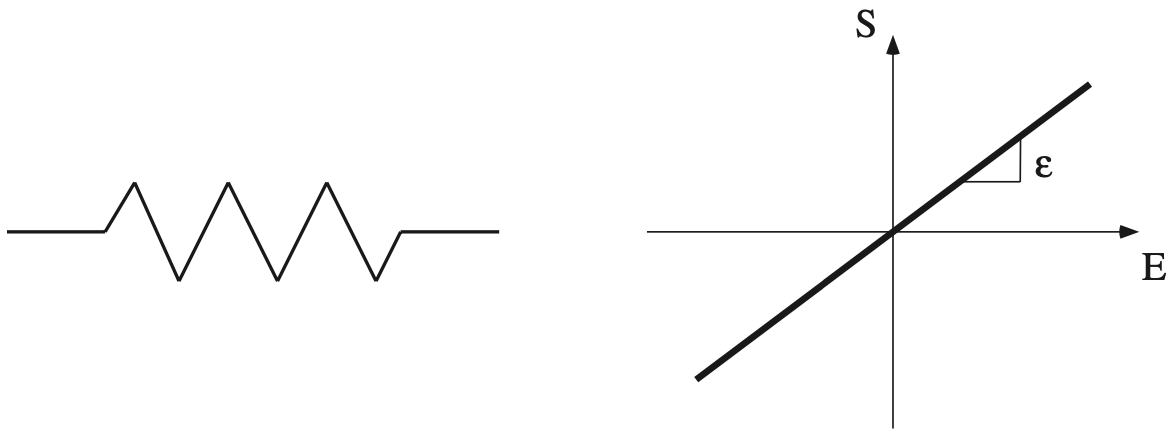
\includegraphics[width=0.5\linewidth]{img/Lin} \\
\end{center}

\textbf{Nonlinear Elasticity:} Elastic and monotone constitutive law \\ $\rightarrow$ material non-linearity.
$S(E) = \frac{\epsilon}{3}\left(\frac{\sqrt{2E + 1}-1}{2E + 1})+2E\right)$
\begin{center}
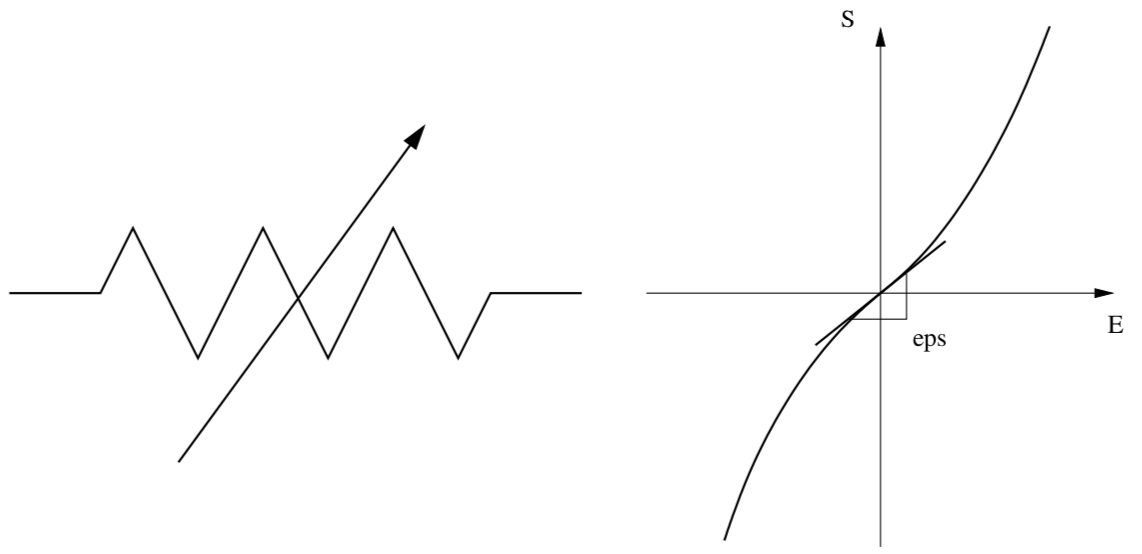
\includegraphics[width=0.5\linewidth]{img/NonLin} \\
\end{center}
\textbf{Geometrical nonlinearity:} linear law with respect to the objective variables is not linear in the nominal variables. \\
$ P(H) = \frac{\epsilon}{2} H (H+1) (H+2)$ induced by the use of material variables! \\

\textbf{Piecewise linear elasticity:} material behaviour law with an elastic modulus that differs in tension and compression.

$S(E) =$
$\begin{cases} 
\epsilon_{-}E, & E \leqslant 0 \\ \epsilon_{+}E, & E \geqslant 0
\end{cases}$

\begin{center}
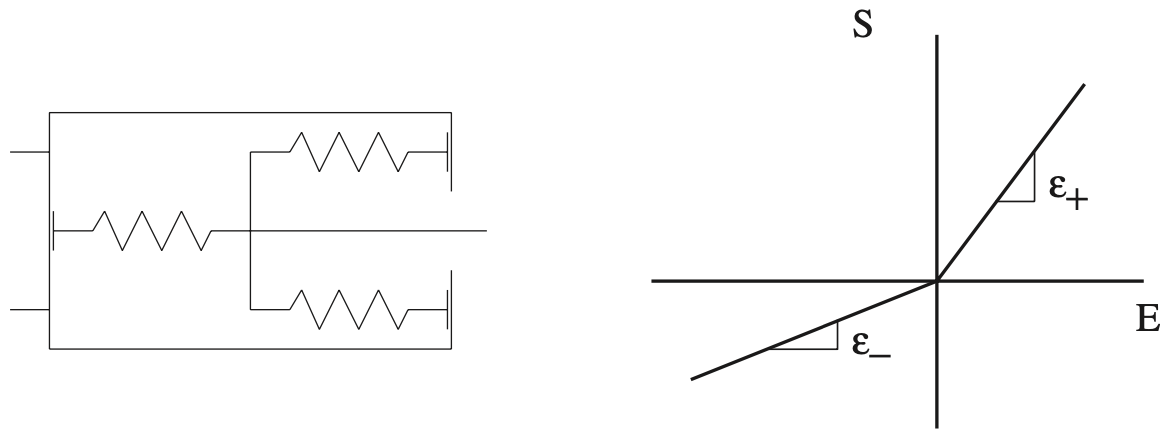
\includegraphics[width=0.5\linewidth]{img/PiecLin} \\
\end{center}



\subsection*{Nonconservative laws}
Cannot be derived from a free energy potential $\rightarrow$ irreversible \\
$\phi \neq 0$ (non-zero dissipation potential). Loading and unloading paths cannot be superimposed in a stress-strain diagram.\\

\textbf{Viscoelasticity:} \\
In Kelvin model, strain remains the only state variable and the total stress is the sum of conservative and dissipative contributions. \\
$\psi (E) = \frac{1}{2} \epsilon E^2$ \qquad $\phi (\dot{E}) =  \frac{1}{2} \mu \dot{E}^2 $ \quad $S(E,\dot{E}) = \epsilon E + \mu \dot{E} $ \\
Where $\epsilon$: elastic module, $\mu$: viscosity coeff. \\

The involved spring and dashpot are independently linear with respect to $E$ and $\dot{E}$, but the total stress is not bilinear with respect to the two variables because they are not independent in a historical sense. Linearity is composed of \textbf{homogeneity} and \textbf{additivity}.

\textbf{Elastoplasticity:} \\
Rate independent, linear elasto-plastic material behavior. Rheologic model: spring with a slider in series. The total deformation is decomposed in elastic+plastic parts.
$E = E^e + E^p$, leading to irreversible strains.

\begin{center}
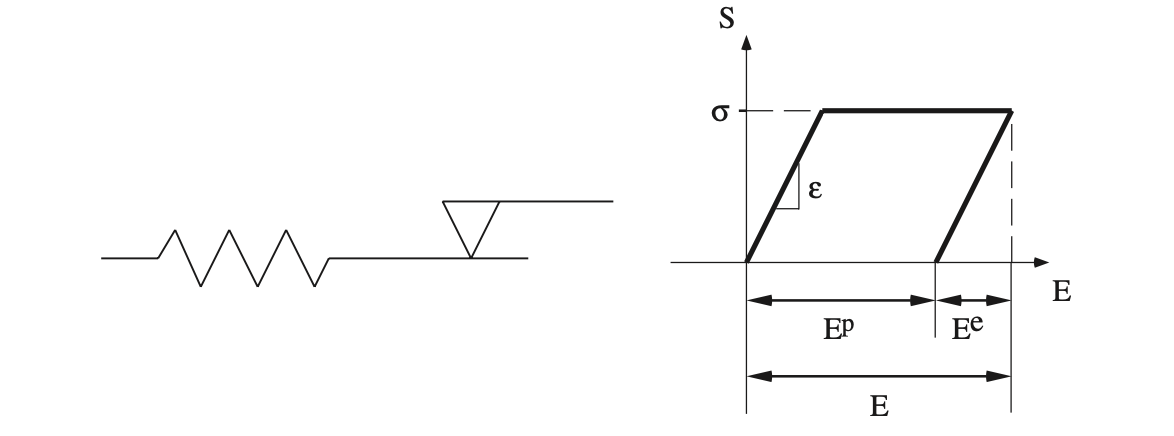
\includegraphics[width=0.5\linewidth]{img/ElastoPlast} \\
\end{center}

\textbf{Damage:} \\
A damaged material has a memory in form of a reduction of its elastic properties $\epsilon$ and can be modelled with the help of an internal variable D, that represents the relative surface occupied by defects or fissures. Elasticity of the tissue is altered but no residual deformation is accounted for. \\
Rheological model: $\tilde{S} = \frac{S}{1-D}$ \\
Corresponding stresses: $S (E,D) = \epsilon (1-D) E,$ \qquad $S^D (E,D) = \frac{1}{2} \epsilon E^2$

\begin{center}
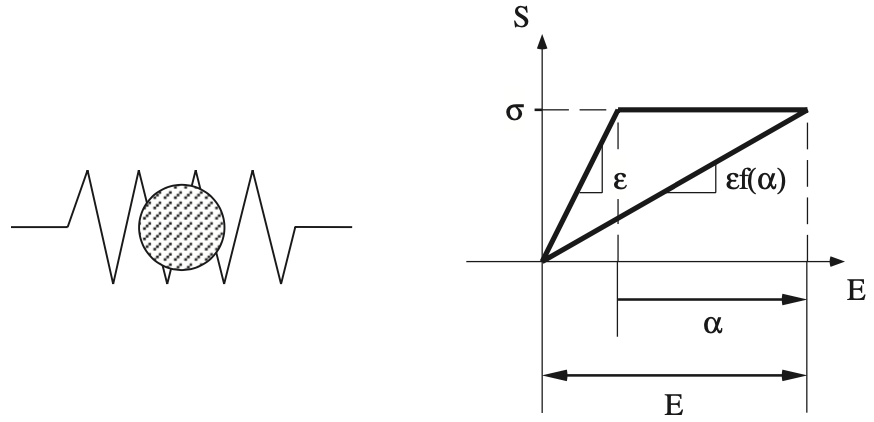
\includegraphics[width=0.5\linewidth]{img/Damage} \\
Rate independent perfect damage
\end{center}
\smallskip
\section{Equilibrium and Thermodynamics}
\subsection*{Equilibrium equations}
\smallskip

\textbf{Divergence theorem} \\
Relates a surface integral with a volume integral.
The \textit{Flux integral} measures the flow rate through a surface. \\
$\int_{\partial \omega} \underline{\underline{\mathbf{P}}} \underline{\mathbf{n}}dA = \int_\omega \nabla_{\underline{\mathbf{x}}} \underline{\underline{\mathbf{P}}} dV$ \\


\textbf{Global equilibrium} \\
\textit{Inertia:} $\int_\omega \rho(\underline{\mathbf{x}},t) \underline{\mathbf{\ddot{y}}},(\underline{\mathbf{x}},t)dV$ \\
\textit{Volume:} $\int_\omega \underline{\mathbf{\kappa}}(\underline{\mathbf{x}},t) dV$ \\
\textit{Contact:} $\int_{\partial \omega} \underline{\underline{\mathbf{P}}}(\underline{\mathbf{x}},t) \underline{\mathbf{n}}(\underline{\mathbf{x}})dA$ \\

\underline{Equilibrium of forces:} \hspace{12.6mm} $\int_\omega \rho \underline{\mathbf{\ddot{y}}}-\underline{\mathbf{\kappa}}-\nabla_{\underline{\mathbf{x}}} \underline{\underline{\mathbf{P}}}dV= 0$ \\
\underline{Equilibrium of moments:} \hspace{8mm} $\int_\omega \underline{\underline{\underline{\epsilon}}}\underline{\underline{\mathbf{F}}}\underline{\underline{\mathbf{P}}}^T dV = 0$ \\


\textbf{Local equilibrium} \\
Assuming continuity, express laws of balance in differential or local form: \\
$\rho \underline{\mathbf{\ddot{y}}}-\underline{\mathbf{\kappa}}-\nabla_{\underline{\mathbf{x}}} \underline{\underline{\mathbf{P}}} = 0 \hspace{5.75mm} \forall \underline{\mathbf{x}} \in \Omega, \forall t$ \\
$\underline{\underline{\mathbf{F}}}\underline{\underline{\mathbf{P}}}^T - \underline{\underline{\mathbf{P}}}\underline{\underline{\mathbf{F}}}^T = 0 \hspace{8mm} \forall \underline{\mathbf{x}} \in \Omega, \forall t$ \\

The \textit{equilibrium of moments } can be interpreted like a condition of symmetry for the tensors of spatial and material stress: \\
$\underline{\underline{\mathbf{F}}}\underline{\underline{\mathbf{P}}}^T = \underline{\underline{\mathbf{P}}}\underline{\underline{\mathbf{F}}}^T = \underline{\underline{\mathbf{T}}} = 
\underline{\underline{\mathbf{T}}}^T = \underline{\underline{\mathbf{S}}} = \underline{\underline{\mathbf{S}}}^T$ 

\subsection*{Thermodynamical principles}
\smallskip
If the equations of state at equilibrium are sufficient to describe the evolution of the system under any history, the behaviour of the system is \textbf{reversible}.
On the other hand, when the equations of state governing the equilibrium are not sufficient to describe the evolution of the system, the behaviour is \textbf{irreversible}. \\

\textbf{First Principle:} Total energy balance

\begin{center}
\emph{"At every moment the derivative of total energy of the body $\Omega$ is equal to the sum of the power developed by the external forces:"}
\end{center}

$\dot{E}^{tot} (\Omega, t) = \dot{W}^{ext} (\Omega, t) \qquad \forall t$ \qquad with $E^{tot} = E^{int} + E^{kin}$ \\
$\dot{E}^{int} = \int_\Omega \underline{\underline{\mathbf{P}}} : \underline{\underline{\mathbf{\dot{F}}}} dV$ \\
$E^{kin} = \frac{1}{2} \int_\Omega \rho \underline{\mathbf{\dot{y}}}^2 dV$ \\

The time derivative of kinetic energy corresponds to the power developed by inertial forces: \\

$\dot{E}^{kin} = \int_\Omega \rho \underline{\mathbf{\dot{y}}} \underline{\mathbf{\ddot{y}}} dV$ \\

\textbf{Power of external forces:} $E^{vol} + E^{con}$\\

$\int_\Omega \underline{\mathbf{\dot{y}}} \cdot \underline{\kappa} dV + \int_\Gamma \underline{\mathbf{\dot{y}}} \cdot \underline{\mathbf{p}}dA$ \\

\textbf{Conjugacy:} $ \underline{\underline{\mathbf{P}}} : \underline{\underline{\mathbf{\dot{F}}}} = \underline{\underline{\mathbf{S}}} : \underline{\underline{\mathbf{\dot{E}}}} = J \underline{\underline{\mathbf{T}}} : \underline{\underline{\mathbf{D}}}$ \\ ($\underline{\underline{\mathbf{T}}}$: True stress, $\underline{\underline{\mathbf{D}}}$: Deformation rate).

\textbf{Second Principle:} Internal dissipation

$\dot{E}^{int} = \int_\Omega \underline{\underline{\mathbf{P}}} : \underline{\underline{\mathbf{\dot{F}}}} dV = \underbrace{\int_\Omega \dot{\psi} dV}_{\text{Reversible}} + \underbrace{\int_\Omega \Phi dV}_{\text{Irreversible}}$, where $\int_\Omega \Phi dV \geq 0 \forall t$ \\
When material behaviour is purely elastic, $\Phi \equiv 0$. \\


\subsection*{Boundary value problems}
\smallskip

To formulate a solvable boundary value problem, the equilibrium equations have to be completed by 4 elements:
 \begin{enumerate}
 \item Conservation of mass
 \item Constitutive laws
 \item Boundary conditions
 \item Initial conditions
 \end{enumerate}
 
\textbf{Virtual velocity:} $\delta \underline{\mathbf{\dot{u}}}(\underline{\mathbf{x}},t)=\underline{\mathbf{\dot{u}}}(\underline{\mathbf{x}},t)-\underline{\mathbf{\dot{\tilde{u}}}}(\underline{\mathbf{x}},t)$

The virtual velocity $\delta \underline{\mathbf{\dot{u}}}$ is also called a variation of the velocity $\underline{\mathbf{\dot{u}}}$. An integral form of the equilibrium equation of the ensemble of the matter contained in the volume $\Omega$ can be obtained by multiplying the differential form with a virtual velocity and by integrating over the volume of the solid (this equation is a \textbf{scalar}): \\

$\int_\Omega \delta \underline{\mathbf{\dot{u}}} \cdot (\rho \underline{\mathbf{\ddot{u}}}-\underline{\mathbf{\kappa}}-\nabla_{\underline{\mathbf{x}}} \cdot \underline{\underline{\mathbf{P}}})dV= 0
\qquad \forall \delta \underline{\mathbf{\dot{u}}}(\underline{\mathbf{x}},t)$ \\

\begin{center}
\emph{"The principle of virtual powers affirms that the total power developed by $^{ine}f$, $^{vol}f$, $^{con}f$ along an arbitrary field of virtual velocities is zero."}
\end{center}

\textbf{Virtual powers:} \\
$\int_\Omega \delta \underline{\mathbf{\dot{u}}} \cdot \rho \underline{\mathbf{\ddot{u}}} dV - \int_\Omega \delta \underline{\mathbf{\dot{u}}} \cdot \underline{\mathbf{\kappa}} dV + \int_\Omega \nabla \delta \underline{\mathbf{\dot{u}}} : \underline{\underline{\mathbf{P}}}dV - \int_{\Gamma_p} \delta \underline{\mathbf{\dot{u}}} \cdot \underline{\mathbf{p}}dA = 0$ \\
\vfill\null
\columnbreak
\section{Notes}
\notes[10pt]{58}{\columnwidth}

\vspace*{\fill}
\\ SP 2020

\end{multicols*}
\end{document}